\documentclass[aspectratio=169]{beamer}

% Theme and Color Setup
\usetheme{Madrid}
\usecolortheme{whale}
\useinnertheme{rectangles}
\useoutertheme{miniframes}

% Additional Packages
\usepackage[utf8]{inputenc}
\usepackage[T1]{fontenc}
\usepackage{graphicx}
\usepackage{booktabs}
\usepackage{listings}
\usepackage{amsmath}
\usepackage{amssymb}
\usepackage{xcolor}
\usepackage{tikz}
\usepackage{pgfplots}
\pgfplotsset{compat=1.18}
\usetikzlibrary{positioning}
\usepackage{hyperref}

% Custom Colors
\definecolor{myblue}{RGB}{31, 73, 125}
\definecolor{mygray}{RGB}{100, 100, 100}
\definecolor{mygreen}{RGB}{0, 128, 0}
\definecolor{myorange}{RGB}{230, 126, 34}
\definecolor{mycodebackground}{RGB}{245, 245, 245}

\title[Introduction to Machine Learning with Spark]{Week 9: Introduction to Machine Learning with Spark}
\author[J. Doe]{John Doe, Ph.D.}
\institute[University Name]{
  Department of Computer Science\\
  University Name\\
  \vspace{0.3cm}
  Email: email@university.edu\\
  Website: www.university.edu
}
\date{\today}

\begin{document}

\frame{\titlepage}

\begin{frame}[fragile]
    \frametitle{Introduction to Machine Learning with Spark}
    \begin{block}{Overview}
        This slide provides an overview of the significance of machine learning in big data analysis and the capabilities provided by Apache Spark MLlib.
    \end{block}
\end{frame}

\begin{frame}[fragile]
    \frametitle{Importance of Machine Learning in Big Data Analysis}
    \begin{itemize}
        \item \textbf{Definition}: Machine Learning (ML) is a subset of artificial intelligence (AI) that enables systems to learn from data and make predictions or decisions automatically.
        \item \textbf{Relevance}: Traditional data processing methods struggle with the vast amounts of data generated today; ML helps in extracting insights, driving data-informed decision-making.
        \item \textbf{Applications}:
        \begin{itemize}
            \item Customer segmentation for targeted marketing.
            \item Fraud detection in financial transactions.
            \item Predictive analytics for sales and inventory management.
        \end{itemize}
    \end{itemize}
\end{frame}

\begin{frame}[fragile]
    \frametitle{The Role of Apache Spark in Machine Learning}
    \begin{itemize}
        \item \textbf{Overview of Apache Spark}: An open-source distributed computing system that enhances performance through parallel processing.
        \item \textbf{Introducing MLlib}:
        \begin{itemize}
            \item \textbf{What is MLlib?} A scalable machine learning library for classification, regression, clustering, and collaborative filtering.
            \item \textbf{Key Benefits}:
            \begin{itemize}
                \item Speed: In-memory computing for faster processing.
                \item Scalability: Efficient handling of large datasets across clusters.
                \item Ease of Use: High-level APIs available in Python, Java, R, and Scala.
            \end{itemize}
        \end{itemize}
    \end{itemize}
\end{frame}

\begin{frame}[fragile]
    \frametitle{Key Concepts: Data Abstraction & Pipeline Concept}
    \begin{itemize}
        \item \textbf{Data Abstraction}: Spark uses distributed datasets (RDDs) or DataFrames for efficient data operations.
        \item \textbf{Pipeline Concept}: A structured sequence for data preprocessing, model training, and evaluation in MLlib.
        \item \textbf{Example:} Building a recommendation system involves:
        \begin{enumerate}
            \item Data Loading: Load user-item interaction data.
            \item Model Selection: Choose an algorithm (e.g., ALS).
            \item Training: Fit the model using training data.
            \item Evaluation: Assess model accuracy with metrics such as RMSE.
        \end{enumerate}
    \end{itemize}
\end{frame}

\begin{frame}[fragile]
    \frametitle{Illustrative Code Snippet}
    \begin{lstlisting}[language=Python]
from pyspark.ml.recommendation import ALS
from pyspark.sql import SparkSession

# Create Spark session
spark = SparkSession.builder.appName("RecommendationExample").getOrCreate()

# Load data
data = spark.read.csv("user_item_ratings.csv", header=True, inferSchema=True)

# Create ALS model
als = ALS(userCol="userId", itemCol="movieId", ratingCol="rating", coldStartStrategy="drop")
model = als.fit(data)

# Generate recommendations
recommendations = model.recommendForAllUsers(10)
    \end{lstlisting}
\end{frame}

\begin{frame}[fragile]
    \frametitle{Conclusion: The Power of ML and Spark}
    \begin{itemize}
        \item \textbf{Impact}: ML combined with Spark MLlib enhances data analysis capabilities, enabling insight discovery and efficiency.
        \item \textbf{Next Steps}: Explore Spark MLlib functionalities and implement machine learning algorithms effectively.
    \end{itemize}
\end{frame}

\begin{frame}[fragile]
    \frametitle{What is Apache Spark? - Overview}
    \begin{block}{Overview of Apache Spark}
        Apache Spark is an open-source, distributed computing framework designed for speed and ease of use in data processing.
        It facilitates both batch and streaming data processing, making it an essential tool in big data analytics.
    \end{block}
\end{frame}

\begin{frame}[fragile]
    \frametitle{What is Apache Spark? - Architecture}
    \begin{block}{Architecture of Apache Spark}
        \begin{enumerate}
            \item \textbf{Components:}
                \begin{itemize}
                    \item \textbf{Driver Program:} The main program that runs your Spark application and converts code into jobs.
                    \item \textbf{Cluster Manager:} Manages resources across a cluster, enabling Spark to utilize various resources (e.g., Spark Standalone, Apache Mesos, Hadoop YARN).
                    \item \textbf{Workers/Executors:} Nodes that perform computations and store data in memory for fast access.
                \end{itemize}

            \item \textbf{Resilient Distributed Datasets (RDDs):}
                \begin{itemize}
                    \item Fundamental data structure in Spark, designed for parallel processing across a cluster.
                    \item RDDs are immutable, fault-tolerant, and can be created from existing data or transformations.
                \end{itemize}
        \end{enumerate}
    \end{block}
    \vspace{0.5cm}
    \begin{center}
        \includegraphics[width=\linewidth]{spark_architecture_diagram.png}  % Please replace with the correct diagram file if available
    \end{center}
\end{frame}

\begin{frame}[fragile]
    \frametitle{What is Apache Spark? - Benefits and Use Case}
    \begin{block}{Benefits of Using Apache Spark}
        \begin{itemize}
            \item \textbf{Speed:} In-memory caching and optimized execution surpass traditional MapReduce frameworks.
            \item \textbf{Ease of Use:} APIs in multiple languages (Scala, Python, Java, R) and the interactive Spark Shell.
            \item \textbf{Versatility:} Supports batch processing, interactive queries, real-time analytics, and machine learning (Spark SQL, Spark Streaming, MLlib).
            \item \textbf{Scalability:} Handles vast data across clusters, facilitating horizontal scalability.
        \end{itemize}
    \end{block}
    
    \begin{block}{Example Use Case}
        \textbf{Case Study: Real-time Data Processing}
        \begin{itemize}
            \item A retail company uses Apache Spark to analyze customer transaction data in real-time.
            \item By processing streaming data with Spark Streaming, the company identifies trends and customer preferences instantly, allowing tailored marketing strategies.
        \end{itemize}
    \end{block}
\end{frame}

\begin{frame}[fragile]
    \frametitle{Overview of MLlib}
    \begin{block}{What is MLlib?}
        MLlib is Apache Spark's scalable machine learning library designed for big data analytics. It enables efficient model building on large datasets for developers and data scientists.
    \end{block}
\end{frame}

\begin{frame}[fragile]
    \frametitle{Key Features of MLlib}
    \begin{itemize}
        \item \textbf{Scalability:} Built on Spark's core, allowing for rapid processing of vast datasets.
        \item \textbf{Unified Framework:} Supports tasks like classification, regression, clustering, and collaborative filtering.
        \item \textbf{Ease of Use:} High-level APIs available in Scala, Java, Python, and R for quick prototyping.
        \item \textbf{Flexibility:} Seamless integration with Spark SQL and DataFrames for structured data access.
    \end{itemize}
\end{frame}

\begin{frame}[fragile]
    \frametitle{Core Components of MLlib}
    \begin{enumerate}
        \item \textbf{Algorithms:} 
            \begin{itemize}
                \item Classification: Logistic regression, Decision trees
                \item Regression: Linear regression, Support vector machines
                \item Clustering: K-means, Gaussian mixture models
                \item Collaborative Filtering: Alternating least squares for recommendations
            \end{itemize}
        \item \textbf{Utilities:} 
            \begin{itemize}
                \item Feature Extraction: Tools like TF-IDF and word2vec
                \item Model Evaluation: Functions to assess model performance
            \end{itemize}
        \item \textbf{Pipelines:} Workflow for machine learning processes, enabling experimentation and model tuning.
    \end{enumerate}
\end{frame}

\begin{frame}[fragile]
    \frametitle{Example Use Case of MLlib}
    \textbf{Predictive Maintenance:} \\
    In industry, MLlib can predict equipment failures using machine learning models based on usage patterns and failure histories.
    
    \begin{lstlisting}[language=Python]
from pyspark.ml.classification import LogisticRegression
from pyspark.ml import Pipeline

# Sample data preparation
data = spark.read.csv("maintenance_data.csv", header=True)

# Define the model
lr = LogisticRegression(featuresCol='features', labelCol='label')

# Build the pipeline
pipeline = Pipeline(stages=[lr])

# Fit the model
model = pipeline.fit(data)
    \end{lstlisting}
\end{frame}

\begin{frame}[fragile]
    \frametitle{Visualizing MLlib}
    \begin{block}{MLlib Workflow Diagram}
        Consider including a flowchart illustrating the MLlib workflow:
        \begin{itemize}
            \item Data Input
            \item Preprocessing
            \item Model Training
            \item Evaluation
            \item Prediction
        \end{itemize}
    \end{block}
\end{frame}

\begin{frame}[fragile]
    \frametitle{Key Takeaways}
    \begin{itemize}
        \item MLlib simplifies machine learning for big data with built-in scalability and high-level APIs.
        \item Supports a variety of machine learning tasks, making it versatile for diverse applications.
        \item Understanding MLlib's components is crucial for effective implementation of machine learning solutions.
    \end{itemize}
\end{frame}

\begin{frame}[fragile]
    \frametitle{Core ML Concepts}
    In this slide, we will explore three fundamental machine learning concepts: 
    \begin{itemize}
        \item **Supervised Learning**
        \item **Unsupervised Learning**
        \item **Reinforcement Learning**
    \end{itemize}
    Understanding these concepts is crucial for leveraging Spark's MLlib in big data scenarios.
\end{frame}

\begin{frame}[fragile]
    \frametitle{1. Supervised Learning}
    \begin{block}{Definition}
        Supervised learning involves training an algorithm using labeled data, mapping input features to correct output labels.
    \end{block}
    
    \begin{itemize}
        \item \textbf{Objective:} Make predictions based on known outcomes.
        \item \textbf{Common Algorithms:} 
            \begin{itemize}
                \item Linear Regression
                \item Decision Trees
                \item Support Vector Machines (SVM)
                \item Neural Networks
            \end{itemize}
    \end{itemize}
    
    \begin{block}{Example}
        \textbf{Spam Detection:} 
        Email data is labeled as "Spam" or "Not Spam." The algorithm learns to classify emails by analyzing features such as sender and keywords.
    \end{block}
\end{frame}

\begin{frame}[fragile]
    \frametitle{2. Unsupervised Learning}
    \begin{block}{Definition}
        Unsupervised learning involves training an algorithm on data without labeled responses, focusing on identifying patterns and structures.
    \end{block}
    
    \begin{itemize}
        \item \textbf{Objective:} Identify intrinsic structures or groupings in data.
        \item \textbf{Common Algorithms:} 
            \begin{itemize}
                \item K-Means Clustering
                \item Hierarchical Clustering
                \item Principal Component Analysis (PCA)
            \end{itemize}
    \end{itemize}
    
    \begin{block}{Example}
        \textbf{Customer Segmentation:} 
        Retail data is analyzed to group customers based on purchasing behavior without predefined labels.
    \end{block}
\end{frame}

\begin{frame}[fragile]
    \frametitle{3. Reinforcement Learning}
    \begin{block}{Definition}
        Reinforcement learning (RL) involves an agent taking actions in an environment to maximize cumulative reward, learning from the consequences rather than direct supervision.
    \end{block}
    
    \begin{itemize}
        \item \textbf{Objective:} Learn optimal actions through trial and error.
        \item \textbf{Common Algorithms:} 
            \begin{itemize}
                \item Q-Learning
                \item Deep Q-Networks (DQN)
            \end{itemize}
    \end{itemize}
    
    \begin{block}{Example}
        \textbf{Game Playing:} 
        A bot learns chess strategies by playing multiple games, receiving rewards for winning and penalties for losing. 
    \end{block}
\end{frame}

\begin{frame}[fragile]
    \frametitle{Conclusion}
    These core ML concepts form the foundation for building intelligent systems using Spark. 
    \begin{itemize}
        \item By understanding them, we can effectively apply Spark's MLlib to complex problems in big data environments.
    \end{itemize}
    \begin{block}{Additional Notes}
        Consider including a diagram that illustrates the relationships and differences between the three learning types.
    \end{block}
\end{frame}

\begin{frame}[fragile]
    \frametitle{Data Preprocessing in Spark - Introduction}
    \begin{block}{Introduction}
        Data preprocessing is a critical step in the machine learning workflow, especially when working with large datasets in Spark. This phase involves cleaning, transforming, and preparing data to ensure that it is suitable for analysis and model training.
    \end{block}
\end{frame}

\begin{frame}[fragile]
    \frametitle{Data Preprocessing in Spark - Part 1: Data Cleaning}
    \begin{block}{Data Cleaning}
        \textbf{Definition:} The process of correcting or removing inaccurate, corrupted, or incomplete records from the dataset.
        
        \textbf{Common Techniques:}
        \begin{itemize}
            \item \textbf{Handling Missing Values:}
                \begin{itemize}
                    \item \textbf{Drop Rows:} Use \texttt{DataFrame.dropna()} in Spark.
                    \item \textbf{Imputation:} Fill missing values using \texttt{DataFrame.fillna()}.
                    \begin{lstlisting}
                    df_cleaned = df.dropna()
                    df_filled = df.fillna(0)
                    \end{lstlisting}
                \end{itemize}
            \item \textbf{Removing Duplicates:}
                \begin{itemize}
                    \item Use \texttt{DataFrame.dropDuplicates()} to eliminate duplicates.
                    \begin{lstlisting}
                    df_unique = df.dropDuplicates()
                    \end{lstlisting}
                \end{itemize}
        \end{itemize}
    \end{block}
\end{frame}

\begin{frame}[fragile]
    \frametitle{Data Preprocessing in Spark - Part 2: Data Transformation and Preparation}
    \begin{block}{Data Transformation}
        \textbf{Purpose:} Modify data to improve quality for analysis.
        \begin{itemize}
            \item \textbf{Data Type Conversion:}
                \begin{lstlisting}
                df_transformed = df.withColumn("age", col("age").cast("integer"))
                \end{lstlisting}
            \item \textbf{Feature Engineering:} Extracting new features enhances model performance.
                \begin{lstlisting}
                df_with_year = df.withColumn("year", year(col("date_column")))
                \end{lstlisting}
        \end{itemize}
    \end{block}

    \begin{block}{Data Preparation}
        \textbf{Objective:} Final stage before model training.
        \begin{itemize}
            \item \textbf{Data Partitioning:}
                \begin{lstlisting}
                train_df, test_df = df.randomSplit([0.8, 0.2])
                \end{lstlisting}
            \item \textbf{SQL Operations:} Filter and aggregate data efficiently.
                \begin{lstlisting}
                spark.sql("SELECT * FROM table WHERE age > 30")
                \end{lstlisting}
        \end{itemize}
    \end{block}
\end{frame}

\begin{frame}[fragile]
    \frametitle{Feature Engineering}
    \begin{block}{Overview of Feature Engineering}
        Feature Engineering is a crucial step in the machine learning pipeline, particularly in big data environments like Apache Spark. It involves selecting, modifying, creating, or extracting features that are relevant to the predictive model.
    \end{block}
    \begin{block}{Importance of Feature Engineering}
        \begin{itemize}
            \item Improved Model Performance
            \item Reduction of Overfitting
            \item Dimensionality Reduction
            \item Facilitation of Interpretability
        \end{itemize}
    \end{block}
\end{frame}

\begin{frame}[fragile]
    \frametitle{Importance of Feature Engineering - Details}
    \begin{enumerate}
        \item \textbf{Improved Model Performance}:
        \begin{itemize}
            \item Relevant features lead to better predictions.
            \item Example: In predicting house prices, features like location and square footage matter more than just the house age.
        \end{itemize}

        \item \textbf{Reduction of Overfitting}:
        \begin{itemize}
            \item Appropriate features simplify the model and lessen overfitting risks.
            \item Example: Irrelevant features may cause the model to learn noise instead of trends.
        \end{itemize}

        \item \textbf{Dimensionality Reduction}:
        \begin{itemize}
            \item Techniques can reduce the number of features while preserving dataset essence.
            \item Example: Extracting day of the week and month from individual dates in time series data.
        \end{itemize}

        \item \textbf{Facilitation of Interpretability}:
        \begin{itemize}
            \item Features can provide insights into data and model behavior.
            \item Example: A 'satisfaction score' reflects customer sentiment from multiple survey items.
        \end{itemize}
    \end{enumerate}
\end{frame}

\begin{frame}[fragile]
    \frametitle{Implementing Feature Engineering in Spark}
    \begin{block}{1. Using Spark DataFrames}
    \begin{lstlisting}[language=Python]
from pyspark.sql import SparkSession
from pyspark.sql.functions import col, when

spark = SparkSession.builder.appName("Feature Engineering").getOrCreate()
data = spark.read.csv("data.csv", header=True, inferSchema=True)

# Creating a new feature "total_rooms"
data = data.withColumn("total_rooms", col("bedrooms") + col("bathrooms"))

# Binarizing a categorical feature
data = data.withColumn("high_income", when(col("income") > 100000, 1).otherwise(0))
    \end{lstlisting}
    \end{block}

    \begin{block}{2. Feature Transformation}
        \begin{itemize}
            \item Normalization
            \begin{lstlisting}[language=Python]
from pyspark.ml.feature import MinMaxScaler

scaler = MinMaxScaler(inputCol="rawFeatures", outputCol="scaledFeatures")
scalerModel = scaler.fit(data)
scaledData = scalerModel.transform(data)
            \end{lstlisting}

            \item One-Hot Encoding
            \begin{lstlisting}[language=Python]
from pyspark.ml.feature import OneHotEncoder, StringIndexer

indexer = StringIndexer(inputCol="category", outputCol="categoryIndex")
model = indexer.fit(data)
dataCategory = model.transform(data)

encoder = OneHotEncoder(inputCols=["categoryIndex"], outputCols=["category_ohe"])
data = encoder.fit(dataCategory).transform(data)
            \end{lstlisting}
        \end{itemize}
    \end{block}
\end{frame}

\begin{frame}[fragile]
    \frametitle{Key Takeaways and Conclusion}
    \begin{block}{Key Points to Remember}
        \begin{itemize}
            \item Feature Engineering requires domain knowledge and an understanding of the data.
            \item Iterative improvement of features is essential for model performance.
            \item Spark provides powerful tools for efficient feature manipulation in large datasets.
        \end{itemize}
    \end{block}
    
    \begin{block}{Conclusion}
        Feature Engineering is pivotal for the success of machine learning models, especially in large-scale data environments. Utilizing Spark for feature engineering can significantly enhance machine learning outcomes.
    \end{block}
\end{frame}

\begin{frame}[fragile]
    \frametitle{Model Training in Spark - Overview}
    \begin{block}{Understanding Model Training in Spark with MLlib}
        - **MLlib** is Spark's scalable machine learning library, offering implementations for:
        \begin{itemize}
            \item Classification
            \item Regression
            \item Clustering
            \item Collaborative Filtering
        \end{itemize}
    \end{block}
\end{frame}

\begin{frame}[fragile]
    \frametitle{Model Training in Spark - Algorithms}
    \begin{block}{Key Algorithms Provided by MLlib}
        \begin{enumerate}
            \item \textbf{Classification Algorithms}
                \begin{itemize}
                    \item Logistic Regression: Binary classification.
                    \item Decision Trees: Non-parametric; model based on features.
                    \item Random Forest: Ensemble of trees for improved accuracy.
                \end{itemize}
            \item \textbf{Regression Algorithms}
                \begin{itemize}
                    \item Linear Regression: Relationship modeling.
                    \item Gradient-Boosted Trees (GBTs): Combines weak learners.
                \end{itemize}
            \item \textbf{Clustering Algorithms}
                \begin{itemize}
                    \item K-Means: Groups data into clusters based on similarity.
                    \item LDA: Topic modeling in documents.
                \end{itemize}
            \item \textbf{Collaborative Filtering}
                \begin{itemize}
                    \item Alternating Least Squares (ALS): Recommendation systems.
                \end{itemize}
        \end{enumerate}
    \end{block}
\end{frame}

\begin{frame}[fragile]
    \frametitle{Model Training in Spark - Evaluation Metrics}
    \begin{block}{Evaluation Metrics for Model Performance}
        - **Accuracy**: Correctly predicted instances / Total instances
        - **Precision**: \(\frac{TP}{TP + FP}\)
        - **Recall**: \(\frac{TP}{TP + FN}\)
        - **F1 Score**: \(F1 = 2 \times \frac{(Precision \times Recall)}{(Precision + Recall)}\)
        - **Area Under the ROC Curve (AUC-ROC)**: Distinguishes between classes.
        - **Mean Squared Error (MSE)**: \(\frac{1}{n} \sum (y_i - \hat{y_i})^2\)
    \end{block}
\end{frame}

\begin{frame}[fragile]
    \frametitle{Model Training in Spark - Code Example}
    \begin{block}{Training a Logistic Regression Model in Spark}
        \begin{lstlisting}[language=Python]
from pyspark.ml.classification import LogisticRegression
from pyspark.ml import Pipeline

# Load data
trainingData = spark.read.format("libsvm").load("data/mllib/sample_libsvm_data.txt")

# Create instances of Logistic Regression and create pipeline
lr = LogisticRegression(maxIter=10, regParam=0.01)

# Fit the model
model = lr.fit(trainingData)

# Make predictions
predictions = model.transform(testData)
        \end{lstlisting}
    \end{block}
\end{frame}

\begin{frame}[fragile]
    \frametitle{Model Training in Spark - Conclusion}
    \begin{block}{Conclusion}
        - Spark's MLlib provides powerful tools for scalable machine learning.
        - Understanding algorithms and evaluation metrics is crucial for model performance.
        - Select right algorithms based on data characteristics and problem type.
    \end{block}
\end{frame}

\begin{frame}[fragile]
    \frametitle{Model Evaluation Techniques}
    \begin{block}{Introduction}
        In machine learning, evaluating the performance of a model is crucial for understanding its prediction capabilities on unseen data. This presentation discusses key model evaluation techniques such as:
        \begin{itemize}
            \item Cross-Validation
            \item Area Under the Curve (AUC)
            \item Precision
            \item Recall
            \item F1 Score
        \end{itemize}
    \end{block}
\end{frame}

\begin{frame}[fragile]
    \frametitle{1. Cross-Validation}
    \begin{block}{Definition}
        A technique for assessing how a model will generalize to an independent dataset by dividing the data into 'k' subsets or folds.
    \end{block}
    
    \begin{block}{Process}
        \begin{itemize}
            \item Split the data into $k$ folds.
            \item Train on $k-1$ folds and validate on the remaining fold.
            \item Repeat for $k$ iterations and calculate average performance.
        \end{itemize}
    \end{block}

    \begin{block}{Benefits}
        \begin{itemize}
            \item Reliable estimate of model performance.
            \item Helps prevent overfitting.
        \end{itemize}
    \end{block}
    
    \begin{block}{Example}
        In a 5-fold cross-validation, the dataset is split into 5 parts. The model is trained 5 times, each time using 4 parts for training and 1 part for testing.
    \end{block}
\end{frame}

\begin{frame}[fragile]
    \frametitle{2. Area Under the Curve (AUC)}
    \begin{block}{Definition}
        AUC measures the performance of a classification model at various threshold settings, particularly for binary classification.
    \end{block}

    \begin{block}{Interpretation}
        \begin{itemize}
            \item AUC = 0.5: No discrimination capability (random predictions).
            \item AUC = 1: Perfect discrimination between positive and negative classes.
        \end{itemize}
    \end{block}

    \begin{block}{Illustration}
        A plot of True Positive Rate (TPR) vs. False Positive Rate (FPR) results in the ROC curve, and AUC is the area under this curve.
    \end{block}
\end{frame}

\begin{frame}[fragile]
    \frametitle{3. Precision and Recall}
    \begin{block}{Precision}
        \begin{equation}
        \text{Precision} = \frac{TP}{TP + FP}
        \end{equation}
        \begin{itemize}
            \item \\textbf{TP} = True Positives, \\textbf{FP} = False Positives
        \end{itemize}
        \begin{block}{Application}
            Precision is critical in scenarios where the cost of false positives is high (e.g., fraud detection).
        \end{block}
    \end{block}

    \begin{block}{Recall}
        \begin{equation}
        \text{Recall} = \frac{TP}{TP + FN}
        \end{equation}
        \begin{itemize}
            \item \\textbf{FN} = False Negatives
        \end{itemize}
        \begin{block}{Application}
            Recall is vital when the cost of false negatives is high (e.g., medical diagnoses).
        \end{block}
    \end{block}
\end{frame}

\begin{frame}[fragile]
    \frametitle{4. F1 Score}
    \begin{block}{Definition}
        The F1 Score is the harmonic mean of precision and recall:
        \begin{equation}
        F1 = 2 \times \frac{Precision \times Recall}{Precision + Recall}
        \end{equation}
    \end{block}

    \begin{block}{Importance}
        The F1 score is especially useful for uneven class distributions, providing a single measure that reflects both precision and recall.
    \end{block}

    \begin{block}{Key Points to Remember}
        \begin{itemize}
            \item Cross-validation is essential for reliable model evaluation.
            \item AUC provides an aggregate measure of performance across all thresholds.
            \item Precision and Recall address different aspects of model performance.
            \item The trade-off between Precision and Recall is captured by the F1 Score.
        \end{itemize}
    \end{block}
\end{frame}

\begin{frame}
    \frametitle{Applications of Machine Learning in Big Data}
    \begin{block}{Overview}
        Machine Learning (ML) is transforming various industries through the analysis of massive datasets, leveraging frameworks like Spark for efficient processing and insights.
    \end{block}
\end{frame}

\begin{frame}
    \frametitle{Key Applications of Machine Learning Using Spark}
    \begin{enumerate}
        \item \textbf{Fraud Detection}
        \item \textbf{Recommendation Systems}
        \item \textbf{Customer Segmentation}
        \item \textbf{Predictive Maintenance}
    \end{enumerate}
\end{frame}

\begin{frame}
    \frametitle{Fraud Detection}
    \begin{itemize}
        \item \textbf{Concept:} Detect anomalies in transactions to identify fraudulent activities.
        \item \textbf{Example:} Financial institutions analyze transaction data in real-time.
        \item \textbf{Illustration:} A sudden spike in transactions can be flagged as suspicious.
    \end{itemize}
\end{frame}

\begin{frame}
    \frametitle{Recommendation Systems}
    \begin{itemize}
        \item \textbf{Concept:} Predict user preferences based on historical behavior.
        \item \textbf{Example:} E-commerce platforms like Amazon use Spark for product suggestions.
        \item \textbf{Key Algorithm:} Matrix Factorization for personalized recommendations.
    \end{itemize}
\end{frame}

\begin{frame}
    \frametitle{Customer Segmentation}
    \begin{itemize}
        \item \textbf{Concept:} Cluster customers based on purchasing behavior for targeted marketing.
        \item \textbf{Example:} Retailers use Spark's MLlib to segment customers for promotions.
    \end{itemize}
\end{frame}

\begin{frame}
    \frametitle{Predictive Maintenance}
    \begin{itemize}
        \item \textbf{Concept:} Predict equipment failures using historical data.
        \item \textbf{Example:} Manufacturing industries forecast machinery maintenance needs using sensor data.
    \end{itemize}
\end{frame}

\begin{frame}
    \frametitle{Key Points to Emphasize}
    \begin{itemize}
        \item \textbf{Scalability:} Spark enables efficient scaling of ML applications.
        \item \textbf{Real-Time Processing:} Spark Streaming for immediate insights.
        \item \textbf{Diverse Algorithms:} Extensive support in Spark MLlib for various tasks.
        \item \textbf{Integration:} Easy integration with big data tools like Hadoop.
    \end{itemize}
\end{frame}

\begin{frame}[fragile]
    \frametitle{Sample Code Snippet for Fraud Detection}
    \begin{lstlisting}[language=Python]
from pyspark.sql import SparkSession
from pyspark.ml.classification import RandomForestClassifier
from pyspark.ml.feature import VectorAssembler

# Initialize Spark Session
spark = SparkSession.builder.appName("FraudDetection").getOrCreate()

# Load data
data = spark.read.csv("transactions.csv", header=True, inferSchema=True)

# Feature Engineering
feature_columns = ['amount', 'location', 'time']
assembler = VectorAssembler(inputCols=feature_columns, outputCol='features')
train_data = assembler.transform(data)

# Train Random Forest Model
rf = RandomForestClassifier(featuresCol='features', labelCol='label')
model = rf.fit(train_data)
    \end{lstlisting}
\end{frame}

\begin{frame}
    \frametitle{Conclusion}
    Understanding and harnessing ML in big data applications enhances business outcomes and customer satisfaction, making powerful ML capabilities accessible at scale through Spark.
\end{frame}

\begin{frame}[fragile]
    \frametitle{Overview of Key Challenges}
    Machine learning (ML) applications at scale using Apache Spark face several obstacles that can hinder performance, accuracy, and efficiency. Here are the primary challenges:
\end{frame}

\begin{frame}[fragile]
    \frametitle{1. Data Quality}
    \begin{itemize}
        \item \textbf{Explanation:} High-quality data is crucial for effective machine learning.
        \item \textbf{Issues:} 
        \begin{itemize}
            \item Missing values
            \item Incorrect labels
            \item Noisy data
        \end{itemize}
        \item \textbf{Example:} In a customer segmentation dataset, erroneous age values can lead to inaccurate segments.
        \item \textbf{Key Points:}
        \begin{itemize}
            \item Clean and preprocess data using Spark's libraries (e.g., Spark SQL and MLlib).
            \item Implement data validation techniques to ensure integrity.
        \end{itemize}
    \end{itemize}
\end{frame}

\begin{frame}[fragile]
    \frametitle{2. Computational Power}
    \begin{itemize}
        \item \textbf{Explanation:} While Spark is designed for distributed computing, large datasets can stress computational resources.
        \item \textbf{Example:} Training a neural network on a massive dataset like ImageNet may require substantial memory and processing power.
        \item \textbf{Key Points:}
        \begin{itemize}
            \item Utilize Spark's cluster capabilities effectively to balance workloads.
            \item Explore using Spark with GPU-based clusters for deep learning tasks.
        \end{itemize}
    \end{itemize}
\end{frame}

\begin{frame}[fragile]
    \frametitle{3. Algorithm Selection}
    \begin{itemize}
        \item \textbf{Explanation:} Choosing the right algorithm is crucial, especially with big data.
        \item \textbf{Example:} For binary classification, logistic regression may underperform compared to decision trees or ensemble methods.
        \item \textbf{Key Points:}
        \begin{itemize}
            \item Understand the strengths and weaknesses of various Spark MLlib algorithms.
            \item Experiment with multiple algorithms using cross-validation to determine the best fit.
        \end{itemize}
    \end{itemize}
\end{frame}

\begin{frame}[fragile]
    \frametitle{Illustrative Diagram: Spark ML Workflow}
    \begin{center}
        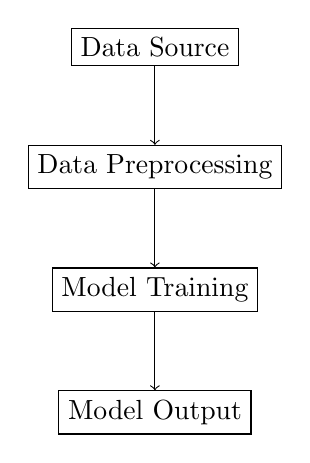
\begin{tikzpicture}
            \node (data) [draw, rectangle] {Data Source};
            \node (preproc) [draw, rectangle, below=1cm of data] {Data Preprocessing};
            \node (train) [draw, rectangle, below=1cm of preproc] {Model Training};
            \node (output) [draw, rectangle, below=1cm of train] {Model Output};
            
            \draw[->] (data) -- (preproc);
            \draw[->] (preproc) -- (train);
            \draw[->] (train) -- (output);
        \end{tikzpicture}
    \end{center}
    \textbf{Note:} Enable monitoring and debugging to understand where challenges may arise during the workflow.
\end{frame}

\begin{frame}[fragile]
    \frametitle{Conclusion}
    Addressing these challenges effectively can significantly improve the performance and reliability of machine learning models developed using Spark, leading to better insights and more robust decision-making in real-world applications.
\end{frame}

\begin{frame}[fragile]
    \frametitle{Future Trends in Machine Learning and Big Data - Introduction}
    Understanding emerging trends in \textbf{Machine Learning (ML)} and \textbf{Big Data} is critical for adapting to technological advancements and optimizing data-driven decision-making processes.
    
    \begin{block}{Key Areas of Discussion}
        - Federated Learning
        - AutoML (Automated Machine Learning)
        - Explainable AI (XAI)
        - Edge Computing
        - Integration of AI and Big Data Analytics
    \end{block}
\end{frame}

\begin{frame}[fragile]
    \frametitle{Key Trends in Machine Learning and Big Data - Part 1}
    \begin{enumerate}
        \item \textbf{Federated Learning}
            \begin{itemize}
                \item \textbf{Explanation:} A decentralized approach to ML where models are trained across multiple devices holding local data samples, without exchanging them.
                \item \textbf{Example:} Used in mobile phones for predictive text and recommendations while preserving user privacy.
            \end{itemize}
        
        \item \textbf{AutoML (Automated Machine Learning)}
            \begin{itemize}
                \item \textbf{Explanation:} Tools that automate the end-to-end process of applying ML, making it accessible to non-experts.
                \item \textbf{Example:} Google Cloud AutoML allows users to train custom ML models without needing deep knowledge of data science.
            \end{itemize}
    \end{enumerate}
\end{frame}

\begin{frame}[fragile]
    \frametitle{Key Trends in Machine Learning and Big Data - Part 2}
    \begin{enumerate}
        \setcounter{enumi}{2}
        \item \textbf{Explainable AI (XAI)}
            \begin{itemize}
                \item \textbf{Explanation:} AI models must provide explanations for their predictions, enhancing transparency and trust.
                \item \textbf{Example:} In healthcare, models must explain how they arrived at a diagnosis.
            \end{itemize}
        
        \item \textbf{Edge Computing}
            \begin{itemize}
                \item \textbf{Explanation:} Processing data closer to where it is generated to minimize latency.
                \item \textbf{Example:} Self-driving cars compute sensor data locally to identify objects and navigate.
            \end{itemize}

        \item \textbf{Integration of AI and Big Data Analytics}
            \begin{itemize}
                \item \textbf{Explanation:} Pairing AI algorithms with big data creates smarter analytics systems.
                \item \textbf{Example:} Retailers analyze consumer behavior using big data and AI to predict trends.
            \end{itemize}
    \end{enumerate}
\end{frame}

\begin{frame}[fragile]
    \frametitle{Future Trends - Key Points and Conclusion}
    \begin{itemize}
        \item \textbf{Ethical AI Development:} Importance of ethical considerations in data use and algorithm transparency.
        \item \textbf{Data Quality Over Quantity:} Emphasis on reliable data; a shift towards understanding data context.
        \item \textbf{Collaboration and Interdisciplinary Approaches:} Favoring collaboration across fields for innovative solutions.
    \end{itemize}
    
    \begin{block}{Conclusion}
        Engagement with these trends in ML and Big Data is crucial for professionals aiming to harness data for innovation, decision-making, and competitive advantage. Organizations must remain informed to leverage these advancements effectively.
    \end{block}
\end{frame}

\begin{frame}[fragile]
    \frametitle{Conclusion and Key Takeaways - Part 1}
    \begin{block}{Integrating Machine Learning and Big Data with Spark}
        \begin{enumerate}
            \item \textbf{Significance of Integration}:
            \begin{itemize}
                \item \textbf{Scalability}: Spark enables processing massive datasets quickly and efficiently with distributed computing.
                \item \textbf{Real-time Analytics}: Machine learning models can be trained on streaming data, vital for applications like fraud detection and recommendation systems.
            \end{itemize}

            \item \textbf{The Power of Machine Learning}:
            \begin{itemize}
                \item Algorithms discover insights from big data patterns, guiding strategies such as marketing optimization based on user behavior predictions.
            \end{itemize}
        \end{enumerate}
    \end{block}
\end{frame}

\begin{frame}[fragile]
    \frametitle{Conclusion and Key Takeaways - Part 2}
    \begin{block}{Example Applications}
        \begin{itemize}
            \item \textbf{Recommendation Engines}: Platforms like Netflix use machine learning for content recommendations from large datasets processed in real-time.
            \item \textbf{Healthcare}: Predictive analytics foresee patient diagnoses and recommend treatments, utilizing Spark's MLlib for analysis.
        \end{itemize}
    \end{block}

    \begin{block}{Key Points}
        \begin{itemize}
            \item The integration of Spark with machine learning is pivotal for processing big data.
            \item Real-world applications highlight competitive advantages gained through this integration.
            \item Tools like Spark MLlib facilitate quick and efficient model building for advanced data analysis.
        \end{itemize}
    \end{block}
\end{frame}

\begin{frame}[fragile]
    \frametitle{Conclusion and Key Takeaways - Part 3}
    \begin{block}{Closing Thoughts on the Future of Data Analysis}
        \begin{itemize}
            \item The combination of machine learning and big data will continue to evolve with new technology advancements.
            \item Expect innovations such as enhanced predictive models and sophisticated real-time processing techniques.
            \item Cross-disciplinary approaches merging domain knowledge with data science will enrich analyses and improve decision-making.
        \end{itemize}
    \end{block}

    \begin{block}{Diagram Idea}
        Display a flowchart illustrating how Spark processes big data and integrates with machine learning algorithms, showcasing the cycle from data ingestion to insight generation.
    \end{block}
\end{frame}


\end{document}